\documentclass[runningheads]{llncs}
%
\usepackage[T1]{fontenc}
\usepackage{graphicx}
\usepackage{tikz}
\usepackage{wrapfig}

\begin{document}
%
\title{A formal approach in train regulation}
%
%\titlerunning{Abbreviated paper title}
% If the paper title is too long for the running head, you can set
% an abbreviated paper title here
%
\author{Guillaume Bonfante \and Martin Vassor  \and Lucas Villaume}
%
\authorrunning{G. Bonfante et al.}
% First names are abbreviated in the running head.
% If there are more than two authors, 'et al.' is used.
%
\institute{Université de Lorraine -- CNRS -- LORIA}
%
\maketitle
%
\begin{abstract}
	...

\keywords{First keyword  \and Second keyword \and Another keyword.}
\end{abstract}


\section{Introduction}
\label{sec:introduction}

This contribution finds its origin in a cyber-warefare we are organising for the IT students at the University of Lorraine, see~\cite{CHE}. In the game-play, we have both IT infrastructures and physical systems, with connections between them. On the physical side, we built a small train network that tries to be a good model of real systems.  Our system manages customer informations, train regulation and finally rail infrastructure. Attackers can hit any of the three parts: disfiguring the site, changing a dock or blocking a light. Defenders will protect their system.

\medskip

\begin{wrapfigure}[6]{r}{0.45\textwidth}
\vspace{-6mm}
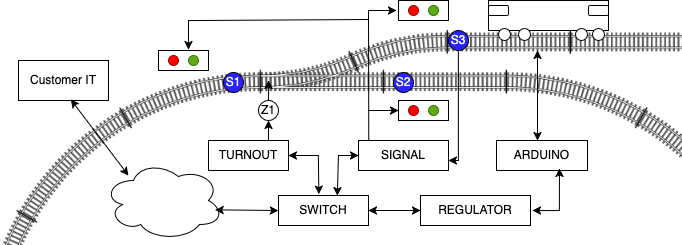
\includegraphics[height=20mm]{TrainSchema.png}
\end{wrapfigure}


From an IT point of view, our system is shaped as shown on the right. We find two databases, one for the customers, one for the infrastructure, switches are controlled by a raspberry (TURNOUT) running an OpenPLC program, signals are controlled by an other raspberry and both communicate via modbus. The SIGNAL automaton read mouvement sensors (not all links shown in the figure). Next to that, we have a third machine, the regulator: it is in charge of updating train routes (as required by the customer IT),  of the regulation of turnouts and finally it may lock some signal (turn it to "red"). All the network connections are done via a single switch, connections from REGULATOR to TURNOUT and SIGNAL are done via modbus while the customer IT and the regulator talks  are based on TCP/IP.  To activate train mouvements, we use the DCC protocol via an Arduino, but this part is strictly related to the fact we have a model train. 


\begin{wrapfigure}[7]{r}{0.3\textwidth}
\hspace{-10mm}
 \begin{minipage}{0.3\textwidth}
        \centering
        \vspace{-24mm}
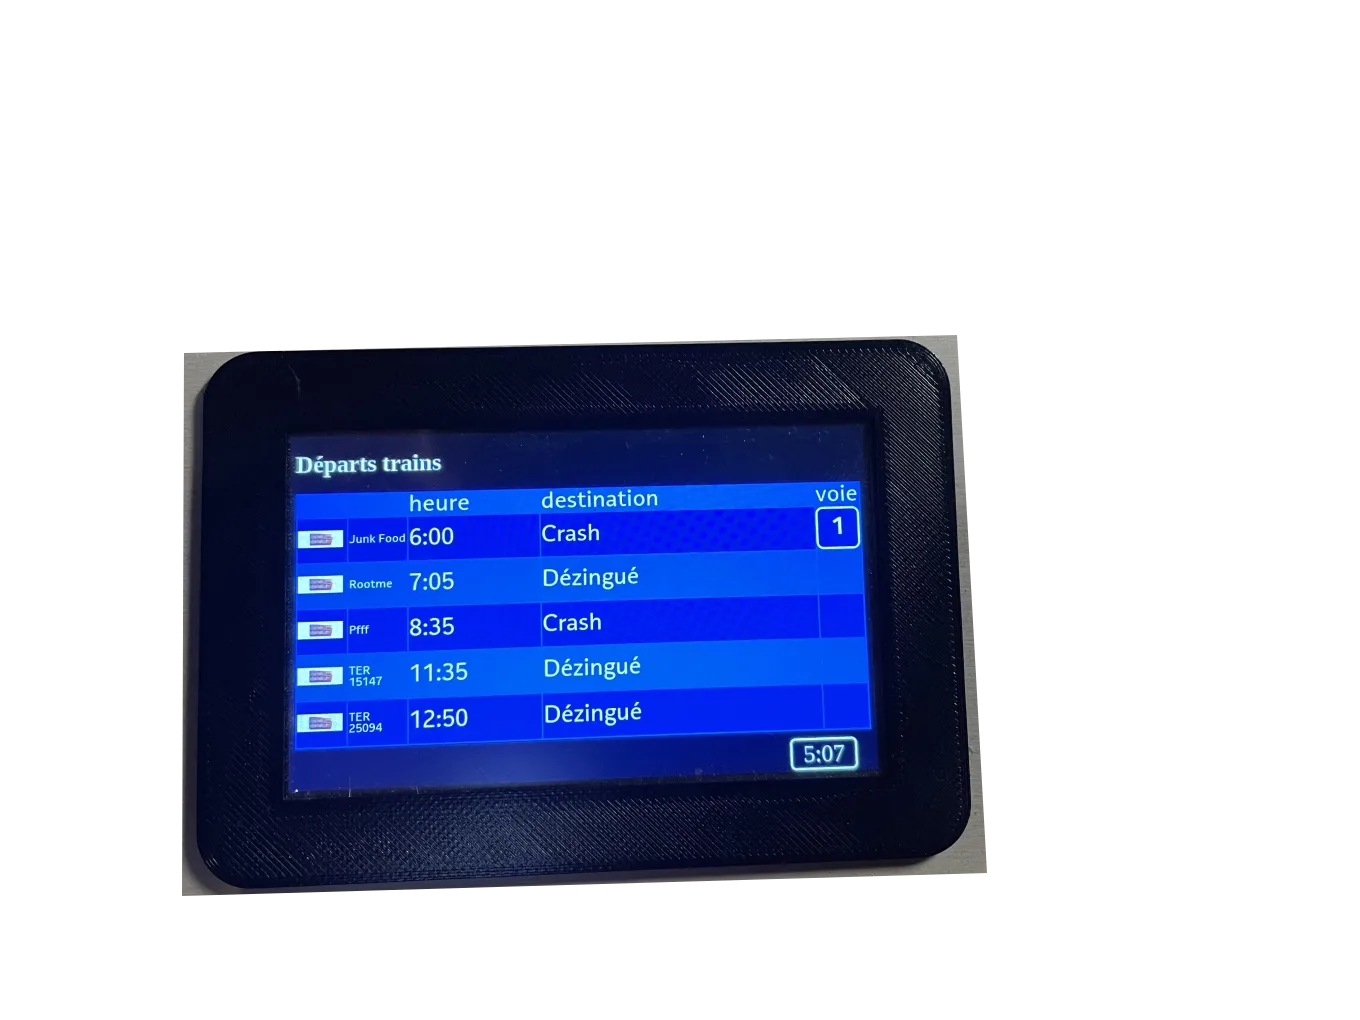
\includegraphics[height=50mm]{ZoomAffichage.png}
    \end{minipage}
\end{wrapfigure}

 The customer IT is deported from the infrastructure (thus the cloud).  It is itself composed of three machines: one for the station screens, one for the databases and a final orchestrator. On the orchestrator, there are two main services: we have a web-service (with front and backend, on the right) and the general route scheduler.  Our model is completely automatic, no manual intervention is needed apart from minor mechanical problems that come with our scale model.
 
 Routes are not computed in advance. The schedule is renewed every "day" and we introduce some randomness in the process: some trains are not the usual ones, some trains departure/destination may change, and so on. In our model, we distinguish freight and  passengers routes giving priority to the latter. 
 
 


% ############################# %
% Espace réservé aux encadrants %
% ############################# %



\section{Modèle informel}
\label{sec:informal-model}

\section{Modèle formel}
\label{sec:formal-model}

\section{Formalisation en TLA}
\label{sec:tla-formalisation}

\section{Composition}
\label{sec:composition}

\section{Expériences}
\label{sec:experiments}

\section{Conclusion}
\label{sec:conclusion}



\bibliographystyle{splncs04}
\bibliography{refs}
\end{document}
